\documentclass[14pt,compress]{beamer}

% Modified from: generic-ornate-15min-45min.de.tex
\mode<presentation>
{
  \usetheme{default}
  %\useoutertheme{infolines}
  \setbeamercovered{invisible}
}

% To remove navigation symbols
\setbeamertemplate{navigation symbols}{}

\usepackage[english]{babel}
\usepackage[latin1]{inputenc}
%\usepackage{times}
\usepackage[T1]{fontenc}
\usepackage{pgf}
\usepackage{amsmath}
\usepackage{movie15}


% Taken from Fernando's slides.
\usepackage{ae,aecompl}
\usepackage{mathpazo,courier,euler}
\usepackage[scaled=.95]{helvet}

\definecolor{darkgreen}{rgb}{0,0.5,0}

\usepackage{listings}
\lstset{language=Python,
  basicstyle=\small\ttfamily,
  commentstyle=\color{red}\itshape,
  stringstyle=\color{darkgreen},
  showstringspaces=false,
  keywordstyle=\color{blue}\bfseries,
  moredelim=**[is][\btHL]{`}{`},
}

%%%%%%%%%%%%%%%%%%%%%%%%%%%%%%%%%%%%%%%%%%%%%%%%%%%%%%%%%%%%%%%%%%%%%%
% Macros
\setbeamercolor{emphbar}{bg=blue!20, fg=black}
\newcommand{\emphbar}[1]
{\begin{beamercolorbox}[rounded=true]{emphbar}
      {#1}
 \end{beamercolorbox}
}
\newcounter{time}
\setcounter{time}{0}
\newcommand{\inctime}[1]{\addtocounter{time}{#1}{\tiny \thetime\ m}}
\newcommand{\inblue}[1]{{\color{blue}#1}}

\newcommand{\typ}[1]{\lstinline{#1}}
\newcommand{\myemph}[1]{\structure{\emph{#1}}}
\newcommand{\PythonCode}[1]{\lstinline{#1}}
\newcommand{\py}[1]{\PythonCode{#1}}

\newcommand{\mysection}[1]{\Large \begin{center}\myemph{#1}\end{center}}

\newcommand{\kwrd}[1]{ \texttt{\textbf{\color{blue}{#1}}}  }

\newcommand\BackgroundPicture[1]{%
  \setbeamertemplate{background}{%
      \parbox[c][\paperheight]{\paperwidth}{%
      \vfill \hfill
        \pgfimage[width=1.0\paperwidth,height=1.0\paperheight,interpolate=true]{#1}
 \hfill \vfill
}}}

% For non-wide pictures, set the width so that the height scales
% appropriately.
\newcommand\BackgroundPictureWidth[1]{%
  \setbeamertemplate{background}{%
      \parbox[c][\paperheight]{\paperwidth}{%
      \vfill \hfill
        \pgfimage[width=1.0\paperwidth,interpolate=true]{#1}
 \hfill \vfill
}}}


% For shorter pictures, set the height so that the width scales
% appropriately.
\newcommand\BackgroundPictureHeight[1]{%
  \setbeamertemplate{background}{%
      \parbox[c][\paperheight]{\paperwidth}{%
      \vfill \hfill
        \pgfimage[height=1.0\paperheight,interpolate=true]{#1}
 \hfill \vfill
}}}


%%%%%%%%%%%%%%%%%%%%%%%%%%%%%%%%%%%%%%%%%%%%%%%%%%%%%%%%%%%%%%%%%%%%%%%%%%%%

\pgfdeclareimage[height=0.75cm]{iitblogo}{iitblogo}
%\logo{\pgfuseimage{iitblogo}}

%% Delete this, if you do not want the table of contents to pop up at
%% the beginning of each subsection:
\AtBeginSubsection[]
{
  \begin{frame}<beamer>
    \frametitle{Outline}
    \Large
    \tableofcontents[currentsection,currentsubsection]
  \end{frame}
}

\AtBeginSection[]
{
  \begin{frame}<beamer>
    \frametitle{Outline}
    \Large
    \tableofcontents[currentsection,currentsubsection]
  \end{frame}
}



%%% Local Variables:
%%% mode: latex
%%% TeX-master: t
%%% End:


\title[Mayavi/VTK]{Mayavi and VTK}
\subtitle{Introduction}
\author[Prabhu]{Prabhu Ramachandran}

\institute[IIT Bombay] {\normalsize
\color{brown}{Department of Aerospace Engineering\\
IIT Bombay}
}
\date[] {
\small
\color{darkgreen}{NGCM Summer School\\
Southampton, UK\\
June 27--28, 2018}
}

%%%%%%%%%%%%%%%%%%%%%%%%%%%%%%%%%%%%%%%%%%%%%%%%%%%%%%%%%%%%%%%%%%%%%%
% DOCUMENT STARTS
\begin{document}

\begin{frame}
  \maketitle
\end{frame}

\begin{frame}
  \frametitle{Outline}
  \Large
  \tableofcontents
  % You might wish to add the option [pausesections]
\end{frame}

\section{Background and Motivation}

\begin{frame}
  \mysection{Visualization?}
\end{frame}

\begin{frame}
  \frametitle{What is visualization?}
  \begin{block}{Visualization: graphics}
    \begin{quote}
      Making a visible presentation of numerical data, particularly a
      graphical one.  This might include anything from a simple X-Y
      graph of one dependent variable against one independent variable
      to a {virtual reality} which allows you to fly around the data.
    \end{quote}
     -- from the Free On-line Dictionary of Computing
  \end{block}
\end{frame}

\begin{frame}
    \frametitle{What is visualization?}
    \Large
    \begin{center}
    Visual representation of data
    \end{center}
\end{frame}


\begin{frame}
    \frametitle{3D visualization}
    \Large
    \begin{center}
        Harder but important
    \end{center}
\end{frame}

\begin{frame}
    \frametitle{Is this Graphics?}
    \Large
    \begin{center}
        Visualization is about data!
    \end{center}
\end{frame}

\begin{frame}[fragile]
    \frametitle{Examples: trajectory in space}
    \Large
\begin{lstlisting}
>>> t = linspace(0, 2*pi, 50)
>>> u = cos(t)*pi
>>> x, y, z = sin(u), cos(u), sin(t)
\end{lstlisting}
\end{frame}

\begin{frame}
    \frametitle{Examples: trajectory in space}
    \Large
    \begin{center}
        \pgfimage[width=2.5in]{MEDIA/m2/mlab/plot3d_ex}
    \end{center}
\end{frame}

\begin{frame}
    \frametitle{Examples: Fire in a room}
    \Large
    \begin{center}
        Demo of data
    \end{center}
\end{frame}

\begin{frame}
  \mysection{Motivation and Needs}
\end{frame}

\begin{frame}
    \Large
    \begin{center}
  Scientists: not interested in graphics

    \end{center}
\end{frame}

\begin{frame}
    \Large
    \begin{center}
   Interactive visualization of data (think Matlab)
    \end{center}
\end{frame}

\begin{frame}
    \Large
    \begin{center}
  Visualization of data files with a nice UI
    \end{center}
\end{frame}

\begin{frame}
    \Large
    \begin{center}
Embedding visualizations in applications
    \end{center}
\end{frame}

\begin{frame}
    \Large
    \begin{center}
        Customization
    \end{center}
\end{frame}

\begin{frame}
    \Huge
    \begin{center}
      \structure{Flexible library/app for every one of these
      needs!}
    \end{center}
\end{frame}


\BackgroundPicture{MEDIA/m2/m2_app3_3.png}
\begin{frame}
\end{frame}
\BackgroundPicture{MEDIA/misc/blank.png}

\begin{frame}[fragile]
  \begin{columns}
    \column{0.62\textwidth}
    \hspace*{-0.45in}
      \footnotesize
\begin{lstlisting}
from mayavi import mlab
from numpy import ogrid
x, y, z = ogrid[-5:5:64j,
                -5:5:64j,
                -5:5:64j]

mlab.contour3d(
    x*x*0.5 + y*y + z*z*2
)
mlab.show()
\end{lstlisting}
    \column{0.4\textwidth}
    \hspace*{-0.1\linewidth}
    \pgfimage[width=1.18\linewidth]{MEDIA/m2/contour3d}
  \end{columns}
\end{frame}

\BackgroundPicture{MEDIA/m2/ipython_mayavi.png}
\begin{frame}[plain]
\end{frame}
\BackgroundPicture{MEDIA/misc/blank.png}

\begin{frame}[plain]
  \begin{center}
    \pgfimage[width=3.25in]{MEDIA/m2/mlab_tui}
  \end{center}
\end{frame}

\BackgroundPicture{MEDIA/m2/lorenz_ui1.png}
\begin{frame}[plain]
\end{frame}

\BackgroundPicture{MEDIA/m2/m2_envisage.png}
\begin{frame}[plain]
\end{frame}
\BackgroundPicture{MEDIA/misc/blank.png}

\BackgroundPictureWidth{MEDIA/m2/mayavi_jupyter.png}
\begin{frame}[plain]
\end{frame}
\BackgroundPicture{MEDIA/misc/blank.png}


\begin{frame}
  \frametitle{Other features}
  \Large
  \begin{itemize}
  \item Automatic script recording
  \item wxPython and Qt support
  \item Powerful command line options
  \item Off-screen support
  \end{itemize}
\end{frame}

\section{Introduction to Mayavi}

\begin{frame}[plain]
  \frametitle{Overview of architecture}
    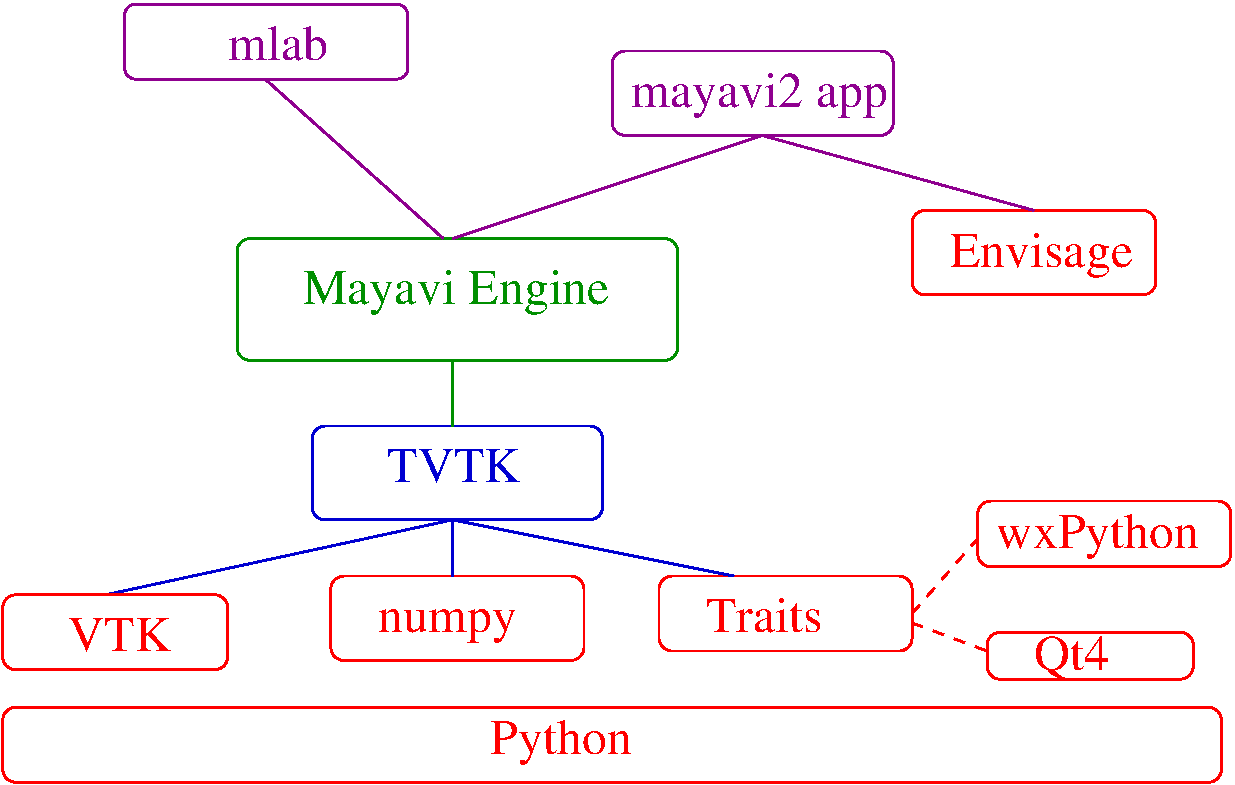
\includegraphics[width=4.25in]{MEDIA/m2/layers.pdf}

\end{frame}


\begin{frame}
  \frametitle{Information}
  \begin{itemize}
  \item \url{http://code.enthought.com/projects/mayavi}
  \item \url{https://github.com/enthought/mayavi}
  \item Uses VTK (\url{www.vtk.org})
  \item BSD license
  \item Linux, Windows and Mac OS X
  \item Debian/Ubuntu/Fedora
  \item Canopy/Anaconda
  \end{itemize}
\end{frame}

\begin{frame}
  \frametitle{Overview of features}
  \begin{itemize}
  \item \typ{mayavi2} application
  \item Python library
  \item OO design
  \item Highly scriptable
  \item \typ{mayavi.mlab}: for easy scripting
  \item \alert{Pythonic}: Seamless NumPy integration
  \item Embed in Traits UIs (wxPython and PyQt4/PySide)
  \item Envisage Plugins
  \end{itemize}
\end{frame}

\subsection{History}

\begin{frame}
    \frametitle{Requirements}
    \Large
    \begin{center}
        Colleagues at IITM needed 3D visualization for CFD data (1998)
    \end{center}
\end{frame}

\BackgroundPicture{MEDIA/m2/4lobe.png}
\begin{frame}[plain]
    \Large
    \begin{center}
    \end{center}
\end{frame}
\BackgroundPicture{MEDIA/misc/blank.png}

\begin{frame}
\Huge
\begin{center}
    \structure{VTK: Visualization Toolkit}
    \vspace*{1in}
    \url{www.vtk.org}
\end{center}
\end{frame}

\begin{frame}
    \Large
    \begin{itemize}
    \item 3D graphics, imaging and visualization
    \item C++ wrappers:  Python (Tcl, Java)
    \item Pipeline architecture
    \item Huge: 900+ classes!
    \item 2000+ classes now!!
    \end{itemize}
\end{frame}

\begin{frame}
    \Large
    \begin{center}
        Who wants to learn a graphics
         library?
    \end{center}
\end{frame}

\begin{frame}
    \frametitle{VTK-CFD (2000)}
    \Large
    \begin{itemize}
        \item Simple UI: Tkinter
        \item Free
    \end{itemize}
\end{frame}

\BackgroundPicture{MEDIA/m2/vtk-cfd/sc1.png}
\begin{frame}[plain]
\end{frame}

\BackgroundPicture{MEDIA/m2/vtk-cfd/sc2.png}
\begin{frame}[plain]
\end{frame}
\BackgroundPicture{MEDIA/misc/blank.png}

\BackgroundPicture{MEDIA/m2/fire_room.png}
\begin{frame}[plain]
\end{frame}
\BackgroundPicture{MEDIA/misc/blank.png}


\BackgroundPicture{MEDIA/m2/fire_vis.png}
\begin{frame}[plain]
\end{frame}
\BackgroundPicture{MEDIA/misc/blank.png}

\begin{frame}
    \frametitle{vtkPipeline}
    \Large
    \begin{center}
    Parse VTK class on the fly producing automatic UI

    \vspace{1in}
    \pause
    Discover and generate VTK pipeline

    \end{center}
\end{frame}

\begin{frame}[fragile]
\vspace*{-6pt}
\normalsize
\begin{lstlisting}
from vtkPipeline import \
vtkPipelineBrowser

# Create a full VTK-Python script
# ...

# renwin is a vtkRenderWindow.
pipe = vtkPipelineBrowser(root, renwin)
pipe.browse ()
\end{lstlisting}
\end{frame}

\begin{frame}
    \Large
    \vspace*{-0.15in}
    \begin{center}
\pgfimage[height=2in]{MEDIA/m2/vtk-cfd/browse}
\pgfimage[height=2in]{MEDIA/m2/vtk-cfd/config}
    \end{center}
\end{frame}

\begin{frame}
    \Large
    \vspace*{-0.15in}
    \begin{center}
\pgfimage[height=3.5in]{MEDIA/m2/vtk_doc}
    \end{center}
\end{frame}

\begin{frame}
    \Large
    \begin{center}
    Doc browser: one afternoon!
    \end{center}
\end{frame}


\begin{frame}
    \frametitle{Lessons}
    \Large
    \begin{itemize}
        \item Python rocks!
        \item VTK is very powerful
    \end{itemize}
\end{frame}

\begin{frame}{Lessons}
    \Large
    \begin{center}
        %\emphbar{
        \begin{itemize}
            \item Run-time introspection
            \item Dynamic programming
            \item Automatic UIs are cool and fun
        \end{itemize}
       %}
    \end{center}
\end{frame}

\begin{frame}{Issues with VTK-CFD}
    \Large
    \begin{center}
        %\emphbar{
        \begin{itemize}
            \item Very specific visualizations
            \item Not general enough
        \end{itemize}
       %}
    \end{center}
\end{frame}

\begin{frame}
\Huge
\begin{center}
    \structure{MayaVi-1.0}
    \vspace*{1in}
    \url{mayavi.sf.net}
\end{center}
\end{frame}

\BackgroundPicture{MEDIA/m2/lox_str_pr.png}
\begin{frame}[plain]
\end{frame}

\BackgroundPicture{MEDIA/m2/mayavi1_demo.png}
\begin{frame}[plain]
\end{frame}
\BackgroundPicture{MEDIA/misc/blank.png}

\begin{frame}
    \Large
    \begin{itemize}
        \item 2001 May
        \item GUI, CLI
        \item One month, including docs
        \item PhD Procrastination Project!
    \end{itemize}
\end{frame}

\begin{frame}{Issues with MayaVi-1.0}
    \Large
    \begin{center}
        %\emphbar{
        \begin{itemize}
            \item No clean scripting API
            \item No MVC
            \item Clunky Tkinter UI
            \item Not easy to embed
        \end{itemize}
       %}
    \end{center}
\end{frame}

\begin{frame}
    \Huge
    \begin{center}
        \structure{Mayavi2}
    \vspace*{0.5in}

    \normalsize
    \url{code.enthought.com/projects/mayavi}

    \vspace*{0.2in}
    2004 --
    \end{center}
\end{frame}

\BackgroundPicture{MEDIA/misc/yoda.jpg}
\begin{frame}[plain]
    \Large
    \begin{center}
        \vspace*{3in}
        {\color{white}{\textbf{Apprentice no longer!}}}
    \end{center}
\end{frame}
\BackgroundPicture{MEDIA/misc/blank.png}

\begin{frame}
    \frametitle{Enthought}
    \Large
    \begin{center}
        TVTK + Mayavi2 (2004)\\
        \vspace*{1in}
    \large
    \url{www.enthought.com}
    \end{center}
\end{frame}

\begin{frame}
    \frametitle{The world of Traits}
    \Large
    \begin{center}
        Python object on steroids!

        \vspace*{1in}
        Part of the Enthought Tool Suite (ETS)
    \end{center}
\end{frame}

\begin{frame}
    \frametitle{TVTK}
    \Large
    \begin{center}
        TVTK = VTK + Traits + NumPy\\
        \vspace*{1in}
        The whole is greater than the sum of the parts!
    \end{center}
\end{frame}

\begin{frame}{Lessons}
    \Large
    \begin{itemize}
        \item The API matters a lot
        \item TDD is quite a life-saver
        \item Be prepared to throw away code!
    \end{itemize}
\end{frame}

\begin{frame}{Mayavi2}
  \Large
  \begin{itemize}
  \item  TVTK + Traits + Envisage
  \end{itemize}
\end{frame}

\begin{frame}
  \frametitle{Recap of architecture}
    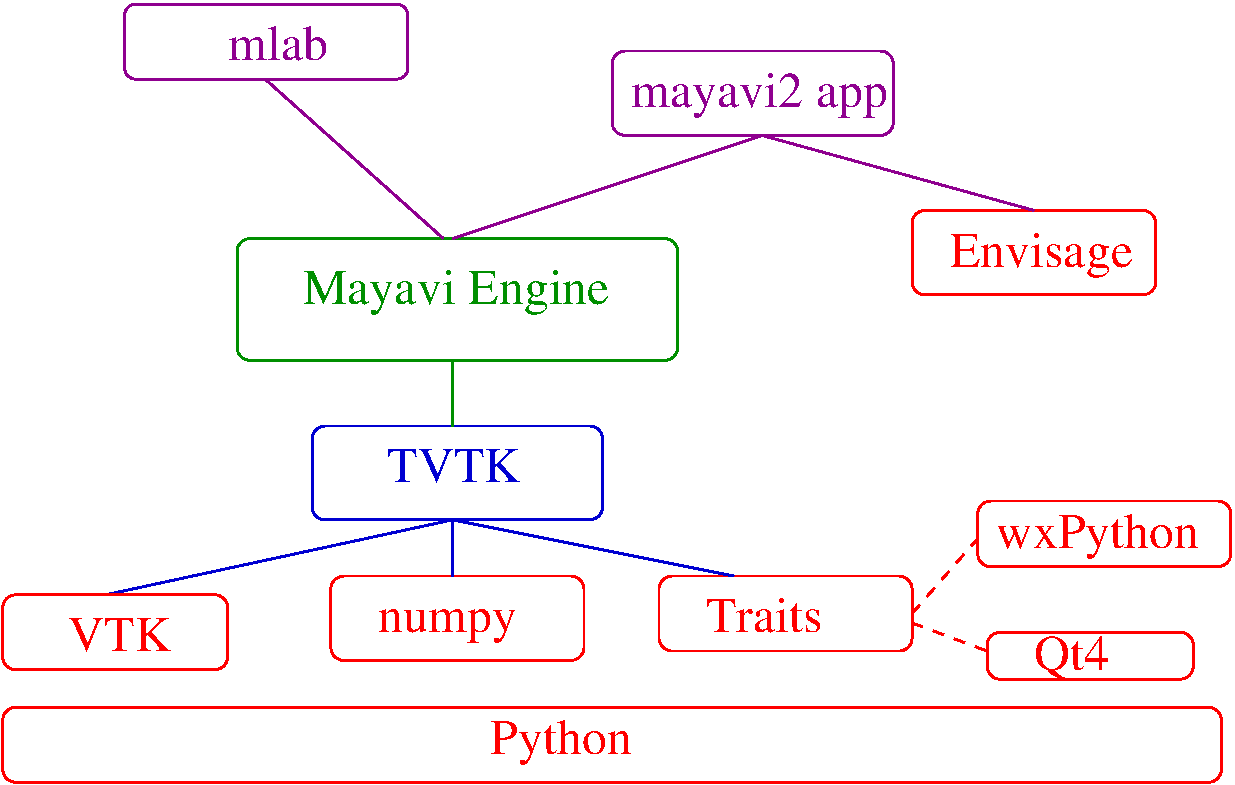
\includegraphics[width=4.25in]{MEDIA/m2/layers.pdf}

\end{frame}

\begin{frame}
  \frametitle{Developers and support}

  \begin{description}[Prabhu Ramachandran]

  \item[Prabhu Ramachandran] Creator and lead, 2001 --

  \item[Ga\"{e}l Varoquaux] Mlab, documentation, usability, 2007 -- 2012

  \item[Enthought Inc.] ETS, Hosting, support, sprints, initial funding,
    distribution

  \item[Deepak Surti] new pipeline support, 2014 -- 2016

  \item[Enthought Devs] Bug fixes, support, testing: Kit Choi, Ioannis Tziakos

  \item[IITB] Freedom and support for PR
  \end{description}

\end{frame}


\end{document}

%%% Local Variables:
%%% mode: latex
%%% TeX-master: t
%%% End:
